\documentclass[a4paper,10pt,twocolumn]{article}

\usepackage[utf8x]{inputenc}
\usepackage[french]{babel}
\usepackage{graphicx,times}
\usepackage[T1]{fontenc}
\usepackage{amsmath}
\usepackage[font=footnotesize]{caption}
\usepackage{fancyhdr}
\usepackage[explicit]{titlesec}
\usepackage{hyperref}
%\usepackage[square,comma,numbers]{natbib}
\usepackage{tabularx}

\newcolumntype{L}[1]{>{\raggedright\arraybackslash}p{#1}}
\newcolumntype{C}[1]{>{\centering\arraybackslash}p{#1}}
\newcolumntype{R}[1]{>{\raggedleft\arraybackslash}p{#1}}

%\renewcommand{\bibsection}{}
%\def\bibfont{\footnotesize}
%\setlength{\bibsep}{0.2em}
%\setlength{\bibhang}{10em}

\hypersetup{colorlinks=true, urlcolor=blue, urlbordercolor={0 0 1}, citecolor=black, citebordercolor={1 1 1}}

\addto\captionsfrench{\def\figurename{Fig.}}
\addto\captionsfrench{\def\tablename{Tableau}}

\captionsetup[figure]{labelsep=period, justification=raggedright, singlelinecheck=false}
\captionsetup[table]{labelsep=period, justification=centering, singlelinecheck=false}

\parindent 10pt

\setlength{\voffset}{-1.3in}
\setlength{\topmargin}{1.25cm}
\setlength{\headheight}{1.125cm}
\setlength{\headsep}{0cm}

\setlength{\hoffset}{-1in}
\setlength{\oddsidemargin}{1.3cm}
\setlength{\evensidemargin}{1.3cm}

\setlength{\textheight}{25cm}%23.5
\setlength{\textwidth}{18.5cm}

\setlength{\headsep}{0.67cm}
\setlength{\columnwidth}{8.75cm}
\setlength{\columnsep}{0.63cm}

\setlength{\abovecaptionskip}{0em}
\setlength{\belowcaptionskip}{0em}

\titleformat{\section}
  {\normalfont}{\thesection.}{0.5em}{\MakeUppercase{#1}}
\titleformat{\subsection}
  {\normalfont\itshape}{\thesubsection.}{1.5em}{#1}
\titleformat{\subsubsection}
  {\normalfont\itshape}{\thesubsubsection.}{1.5em}{#1}
	
\titlespacing\section{0pt}{1em}{0.5em}
\titlespacing\subsection{0pt}{1em}{0.5em}
\titlespacing\subsubsection{0pt}{1em}{0.5em}

\fancyhf{}
\fancyhead[R]{\fontsize{8pt}{8pt}\selectfont \textbf{S}YMPOSIUM DE \textbf{G}ENIE \textbf{E}LECTRIQUE (SGE 2018), 3-5 JUILLET 2018, NANCY, FRANCE}
\renewcommand{\headrulewidth}{0pt}


\pagestyle{empty}


\title{
\fontsize{24pt}{24pt}\selectfont
Gestion d'énergie avec entrées incertaines : \\
quel algorithme choisir ?\\
Maison solaire pour un benchmark open source
}

\newcommand\tsp[1]{\textsuperscript{#1}}

\author{
\fontsize{11pt}{11pt}\selectfont
Pierre HAESSIG\tsp{*}, Jesse James PRINCE AGBODJAN\tsp{*}, Romain BOURDAIS\tsp{*}, Hervé GUÉGUEN\tsp{*}\\
\fontsize{10pt}{10pt}\selectfont
\tsp{*}IETR, CentraleSupélec
}

\date{}


\begin{document}

\maketitle
\thispagestyle{fancy}


\fontsize{9pt}{9pt}\selectfont
\textbf{RÉSUME --
Le pilotage optimal des systèmes énergétiques nécessite l'emploi d'algorithmes
de gestion optimale.
Ces outils se rattachent à théories de disciplines variées (Automatique, Optimisation, Recheche Opérationnelle),
qui ont chacune leur spécificité tout en se recouvrant partiellement.
%
Il est donc difficile, pour la personne ``non-initiée'', de saisir les principales caractéristiques
de chaque approche pour pouvoir les comparer et finalement trouver
quelles méthodes sont plus adaptées à un problème donné.
%
Nous proposons ici, sur un exemple simple de système photovoltaïque-stockage, de
comparer différentes méthodes en soulignant en particulier les investissements
en temps à prévoir :
temps pour la compréhension du cadre théorique,
temps pour la modélisation du problème dans ce cadre,
temps pour l'implémentation numérique et la validation des résultats.
Nous soulignons également quelques pièges typiques, comme l'optimisation
déterministe anticipative dans un contexte stochastique.
}\\

\textbf{\textit{Gestion d'énergie, Optimisation dynamique, Optimisation stochastique,
Commande prédictive, Programmation Dynamique}}

\fontsize{10pt}{10pt}\selectfont


\section{Introduction}

De très nombreux travaux de recherche portent sur le pilotage des systèmes énergétiques
pour optimiser leur fonctionnement.
Les méthodes employées sont variées (cf. partie \ref{s:opt_meth})
et certaines nécessite un bagage théorique qui pourrait rebuter effrayer
une personne issue d'une discipline ``physique'' (génie électrique, énergétique)
plutôt que ``numérique'' (automatique, recherche opérationnelle) où ces méthodes
sont souvent mises au point.
La mise en œuvre peut également est difficile et coûteuse en temps de calcul.
C'est malheureusement le cas en particulier des méthodes
a priori les plus performantes du point de vue de l'optimalité.

En réponse à ces difficultés, nous proposons un \emph{banc de test de gestion d'énergie open source}.
Il permet, sur un exemple simple, mais pertinent, d'avoir un aperçu de différentes méthodes
de pilotage. Cela permet de comparer leur mise en oeuvre (e.g. dans différents langages de programmation)
et leurs résultats (optimalité, robustesse...).

Il existe des travaux comparant des méthodes de gestion d'énergie, sur des exemples réels complexes
(barrages hydroélectriques \cite{Zambelli:2011:SBA}, véhicules hybrides \cite{Jiang:2017:ToVT}).
Notre proposition est complémentaire, car elle porte davantage sur la comparaison \emph{fonctionnelle}
des méthodes (e.g. analyse des objets nécessaires pour leur mise en oeuvre) que
sur la comparaison quantitative des résultats d'optimisation.

\section{Banc de test: maison solaire}

\subsection{Modèle de la maison solaire}

\begin{figure}[!ht]
        \begin{center}
                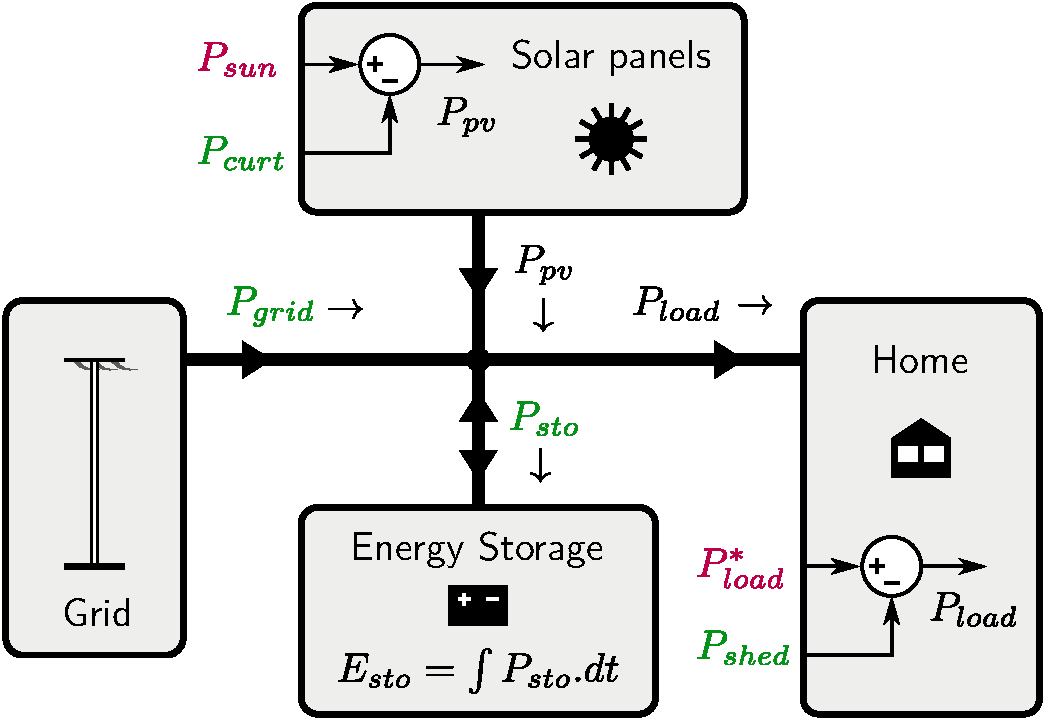
\includegraphics[width=0.9\columnwidth]{figures/solar_home.pdf}
        \end{center}

        \caption{Modèle en flux d'énergie de la maison solaire.
        Variables de décision en vert, données externes en rouge (potentiel solaire et consommation souhaitée), variables internes en noir.
        La consommation du foyer $P_{load}^*$, imposée, est couverte par 3 sources:
        le réseau électrique, des panneaux solaires (délestables)
        et un système de stockage.
        En dernier recours, la consommation de la maison peut être délestée.
        }
        \label{fig:solhome}
\end{figure}

Pour illustrer les différentes méthodes de gestion d'énergie à comparer,
nous avons choisi un système ``banc de test'' qui soit à la fois simple et concret.
Nous considérons ainsi la maison solaire qui est modélisée par
des flux d'énergie figure \ref{fig:solhome}.
Il s'agit d'un modèle simple de système photovoltaïque-stockage
pour l'autoconsommation d'un consommateur résidentiel connecté au réseau.

L'objectif de pilotage est la minimisation de la facture
de l'énergie consommée du réseau ($\int P_{grid}$), le prix de l'énergie étant considéré fixe\footnote{un prix variable serait une extension naturelle}.
La puissance de réseau est limitée à la puissance souscrite $P_{grid}^{max}$
et l'injection est interdite\footnote{
équivalent, du point de vue de l'optimisation, à autoriser l'injection, mais sans la rémunérer}:
%
\begin{equation}
  0 \leq P_{grid} \leq P_{grid}^{max}
\end{equation}
%
Le système de gestion d'énergie doit donc tirer profit de l'énergie, marginalement
gratuite, des panneaux solaires $P_{pv}$, librement réglable entre 0 et $P_{sun}$
(par l'intermédiaire de l'écrêtage $P_{curt} \geq 0$).
$P_{sun}$ est le productible solaire, c'est-à-dire la production des panneaux en régime
MPPT\footnote{Maximum power point tracking}.
Ce productible est fonction de l'irradiance solaire du moment
et de la puissance nominale (puissance crête) des panneaux $P_{pv}^{max}$.

Le système de gestion doit également exploiter le degré de liberté offert par
le système de stockage qui permet de décaler, au moins partiellement,
la production solaire et la consommation. Le stockage, dont on néglige les pertes,
contient l'énergie:

\begin{equation}
  E_{sto}(t) = \int_0^t P_{sto}(t)dt
\end{equation}

Point essentiel, le stockage a une capacité limitée $E_{rated}$ :

\begin{equation}
  0 \leq E_{sto} \leq E_{rated}
\end{equation}

Tous les flux sont liés par la conservation de l'énergie:

\begin{equation}
  P_{grid} + P_{pv} = P_{load} + P_{sto}
\end{equation}

La consommation $P_{load}$ a vocation à suivre la consommation souhaitée $P_{load}^*$
(pas de charges ``intelligentes'' déplaçables). Nous définissons cependant un délestage de dernier
recours pour les situations critiques\footnote{faible puissance souscrite, lorsque
la batterie est vide et qu'il n'y a que peu de soleil}.

Notons pour finir que la performance d'un tel système dépend totalement de son dimensionnement
(capacité de stockage, puissance des panneaux et  puissance souscrite).
La question du dimensionnement, bien qu'intéressante, n'étant pas l'objet de cet article,
le dimensionnement est fixé empiriquement.

Dimensionnement: $E_{rated}=13.5\,$kWh (Tesla Powerwall), $P_{pv}^{max}=3\,$kW\textsubscript{c} (permet, en cumul annuel, de couvrir 64\% de la consommation du foyer présenté ci-après).

\subsection{Banc de test open source}

La description de ce modèle ainsi que les données temporelles nécessaires sont
disponibles en open source dans un dépôt GitHub \href{https://github.com/pierre-haessig/solarhome-control-bench}{solarhome-control-bench}.
Ce dépôt contient également les méthodes de gestion d'énergie présentées dans cet article.

Il a vocation à contenir des exemples dans les langages de programmation les plus utilisés pour ce type de problème:
Matlab, Python et Julia...

\subsection{Données de la maison solaire}

Nous utilisons le jeu de \emph{données réelles et ouvert} ``\href{https://www.ausgrid.com.au/Common/About-us/Corporate-information/Data-to-share/Solar-home-electricity-data.aspx}{Solar home electricity data}'' de l'opérateur Ausgrid (réseau de Sydney et sa région, Australie).
Il contient 3 années de consommation et production, au pas demi-horaire, de 300 clients résidentiels disposants de panneaux PV.

Pour notre banc de test, nous avons sélectionné un client sans charge pilotable\footnote{
  la description détaillée de ce choix est fournie dans le fichier \href{https://github.com/pierre-haessig/solarhome-control-bench/blob/master/data/README.md}{data/README.md} du dépôt, avec plusieurs graphiques supplémentaires.}.
Nous avons choisi 7 jours consécutifs de test représentés figure \ref{fig:testdata} (après mise à l'échelle à 3 kW\textsubscript{c} de son installation PV).

Les données des 30 jours précédents sont également disponibles pour une phase d'apprentissage,
par exemple pour régler la prévision d'une commande prédictive.


\begin{figure}[!ht]
        \begin{center}
                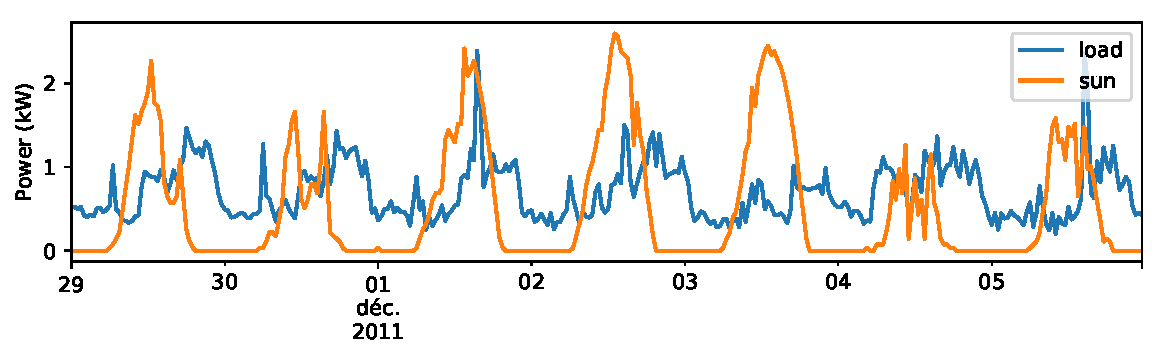
\includegraphics[width=1\columnwidth]{figures/data_week_2011-11-29.pdf}
        \end{center}

        \caption{Consommation et production PV durant les 7 jours de test
        }
        \label{fig:testdata}
\end{figure}


\section{Approches d'optimisation}
\label{s:opt_meth}

L'article final décrira les différentes méthodes comparées pour la gestion de la maison solaire,
avec les résultats obtenus.

\subsection{Programmation dynamique}
Bon cadre théorique pour poser un problème de gestion avec entrées incertaines (stochastique).
Point particulier: nécessite une modélisation des incertitudes par un \emph{processus markovien}\cite{Haessig:2013:ESPy}.
L'implémentation numérique est impossible si la dimension de l'état est trop grande (>4).


\subsection{Optimisation déterministe anticipative}

Un piège courant consiste à optimiser la gestion avec une connaissance parfaite des entrées.
Le résultat (figure \ref{fig:anticip}) est une surévaluation de la performance (e.g. aucun délestage de la production solaire).

%\cite{Rigo-Mariani:2014:SGE}
% poster µgrid powertech 2015 ?

\begin{figure}[!ht]
        \begin{center}
                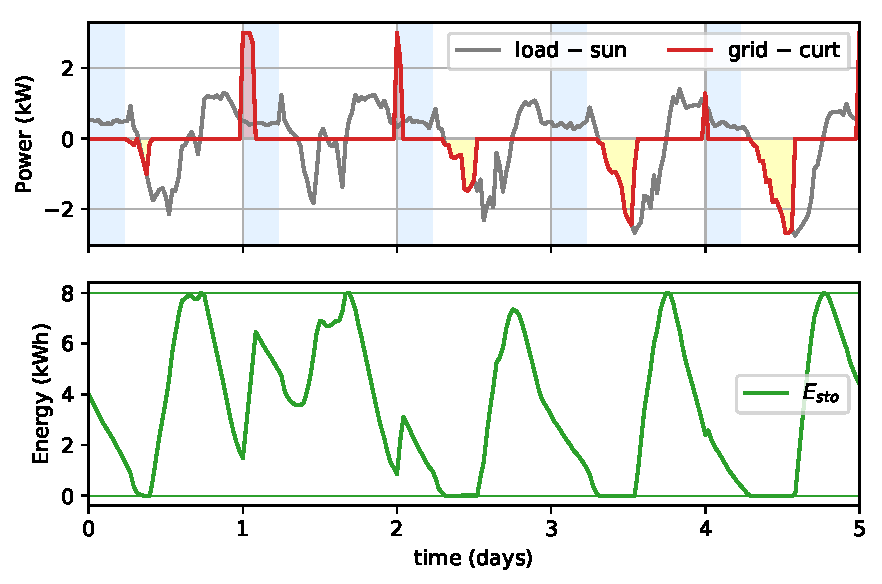
\includegraphics[width=1\columnwidth]{figures/julia_anticipative.pdf}
        \end{center}

        \caption{Gestion d'énergie par optimisation déterministe anticipative. La performance est surestimée
        (aucun délestage de production solaire).
        }
        \label{fig:anticip}
\end{figure}

\subsection{Commande prédictive (MPC)}
La commande prédictive (MPC) utilise une \emph{prévision ponctuelle (moyenne)} des entrées incertaines.
Elle compense l'erreur de prévision en répétant l'optimisation sur un \emph{horizon glissant}.
L'implémentation numérique est efficace si le problème d'optimisation est linéaire (ou en tout cas convexe),
ce qui est le cas ici.

Des variantes du MPC déterministe existent pour mieux faire face à l'incertain: le MPC stochastique,
qui utilise un \emph{ensemble de scénarios}, éventuellement avec un ``recours affine''.

%\subsection{MPC stochastique et robuste}

%une amélioration du MPC déterministe.

% \subsection{Commande prédictive non-linéaire}
% 
% Optimica JModelica.org \cite{Akesson:2010:CCE}
% 
% sareni sge 2014 \cite{Rigo-Mariani:2014:SGE} : optim linéaire puis reprojection.


\section{Conclusions}

Le banc de test pour la gestion d'énergie d'une maison solaire
doit permettre de faciliter l'accès à une palette de méthode de gestion
sur un exemple simple mais réaliste (e.g. données de production solaire et de consommation réelles).

Perspectives : ce banc de test pour la gestion d'énergie,
à dimensionnement fixé, est une première étape pour l'étude des méthodes
de dimensionnement optimal qui prennent en compte l'optimisation de la loi de gestion
\cite{Haessig:2014:SGE}.

% structure de décision dans un contexte multi-agent (pas abordé ici
% car focus sur optimisation d'un système individuel) : centralisé, distribué,
% mécanisme de prix, multi-agent...

\bibliographystyle{IEEEtran}
\bibliography{00_References}

\end{document}